\section{Design}

The game is designed based on the \textbf{Model-View-Controller (MVC)} architecture.
This architecture is a common way of designing applications with a User Interface.
In it, each of the following components is responsible for a particular task, and only that component is allowed to perform that task.

\begin{table}[H]
  \centering
  \bgroup
  \def\arraystretch{1.5}
  \begin{tabularx}{\textwidth}{|p{3cm}|X|}
    \hline
    \multirow{2}{*}{\textbf{Model}}  & This is the part of the framework responsible for maintainin the internal representation of the application.                      \\
                            & The \textbf{Model} in this game holds the location where sand is present, state of each sprite and state variables of the game. \\
    \hline

    \multirow{2}{*}{\textbf{View}}   & The \textbf{View} is responsible for rendering the \textbf{Model} onto the GUI. \\
                            & It contains routines that display the board, the sprites and the sand on a console screen.                                        \\
    \hline

    \multirow{2}{*}{\textbf{Controller}} & The \textbf{Controller} is responsible for handling user input and triggering changes in the \textbf{Model}.\\
                            & It contains the entry point for the game and interrupt handlers. \\
    \hline
  \end{tabularx}
  \egroup
\end{table}


\begin{figure}[H]
  \centering
  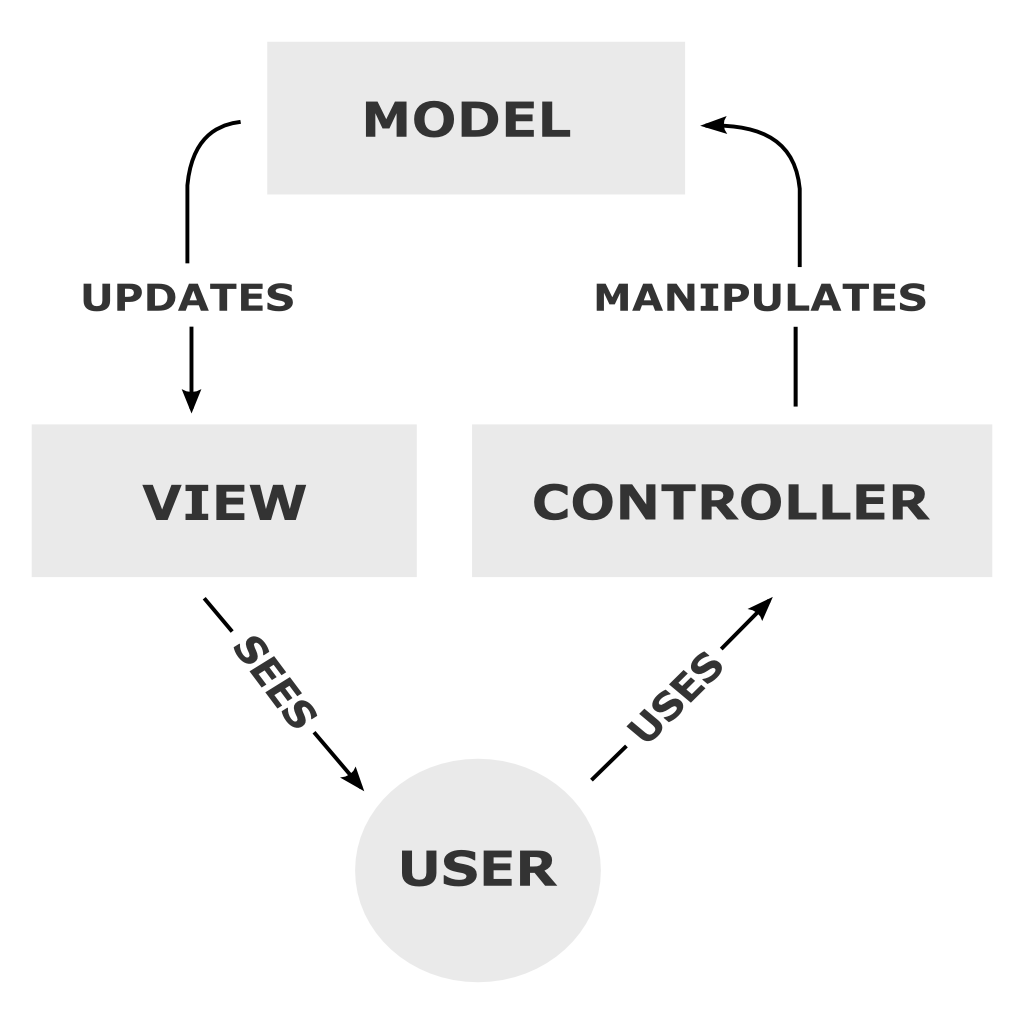
\includegraphics[width=0.5\textwidth]{images/mvc-process.png}
  \caption{\label{fig:mvc-process} The components of the framework interacting with each other (courtsey: Wikipdia)}
\end{figure}


\section{Controller Design}

  \begin{table}[H]
  \begin{tabular}{rl}
    \texttt{FILES}:         &\texttt{controller.s}  \\
    \texttt{WRITTEN BY}:    &\texttt{Anand Balakrishnan (anandbal)}
  \end{tabular}
  \end{table}


  The \textbf{Controller} mainly contains interrupt handlers, and it is also the entry point for the game.
  In is, we do the following:

  \begin{itemize}
    \item Initialize timer and timer match registers for periodic interrupts.
    \item Listen for UART0 interrupt, read the keystrokes and perform the corresponding action.
    \item Listen for External Interrupt Button press and PAUSE the game.
  \end{itemize}

  The \textbf{Controller} is a relatively small component, responsible mainly for updating the \textbf{Model} via subroutines exposed by the \textbf{Model}.



  \section{Model}

  \begin{table}[H]
  \begin{tabular}{rl}
    \texttt{FILES}:         &\texttt{model.s}, \texttt{collisions.s} \\
    \texttt{WRITTEN BY}:    &\texttt{Anand Balakrishnan (anandbal)}
  \end{tabular}
  \end{table}

  The \textbf{Model} maintains the internal representation of the board and triggers \textbf{View} updates. It exposed routines that allows the
  \textbf{Controller} to trigger updates on the \textbf{Model}.

    \subsection{Implementation}

    The \textbf{Model} consists of an \emph{``array''} (created using the \texttt{FILL} directive)
    of size $19 \times 15$ bytes, each byte representing a grain of sand.

    The \textbf{Model} also consists of \texttt{DCD} tables to hold information of sprites. These tables are structured similar to a \texttt{struct}, see \textbf{Listing \ref{lst:sprite-struct}}.
    There are also staticaly defined regions of memory that keep track of the various states the game could possibly be in,
    for example, \texttt{PAUSE}, \texttt{GAME\_OVER}.
    The \textbf{Model} is also responsible for keeping track of other variables of the game,
    such as, \texttt{LEVEL}, \texttt{HIGH\_SCORE}, \texttt{CURRENT\_SCORE} and \texttt{TIME}.


    \begin{lstlisting}[caption={Structure for \texttt{SPRITE} data},label={lst:sprite-struct}]
SPRITE
	DCD X_POS	; Holds X coordinate of the sprite
	DCD Y_POS	; Holds Y coordinate of the sprite
	DCD LIVES	; Holds Number of lives the sprite has
	DCD DIRECTION	; Code for direction the sprite is moving/facing
	DCD OLD_X_POS	; Previous X coordinate of sprite
	DCD OLD_Y_POS	; Previous Y coordinate of sprite
	DCD ORIGINAL_X	; Original X position (to reset when respawning)
	DCD ORIGINAL_Y	; Original Y position (to reset when respawning)

    \end{lstlisting}

    \subsection{Operations}

    Operations that are defined by the \textbf{Model} are:

    \begin{itemize}
      \item Initialize and reset model.
      \item Move sprites and update entire model.
      \item Handle and detect collisions.
      \item Get if sand exists at given (x,y) coordinate on the board.
      \item Clear sand at given coordinate (x,y).
      \item Toggle game states (\texttt{BEGIN\_GAME},\texttt{PAUSE}, \texttt{GAME\_OVER}, \texttt{RUNNING}).
      \item Update individual sprites.
      \item Spawn sprites.
    \end{itemize}

    \subsubsection{Initialize and Reset Model}

    \subsubsection{Game States and Representation}

    \subsubsection{Update Model and Control Sprites}

    \subsubsection{Collision Detection}




  \subsection{View}

  \quad\textbf{FILES}: \texttt{gui.s}, \texttt{peripherals.s}


  The \textbf{View} is responsible for rendering \textbf{Model} onto the GUI. It possessed routines that
  the \textbf{Model} uses to trigger updates to the GUI. This implementation was chosen as updates can
  be triggered as and when the \textbf{Model} is updates.

    \subsubsection{Implementation}





